% Sample content to demonstrate tikzpicture

\chapter{Current State Analysis}

Data to plot the graph \ref{fig:stdplot} are in data.dat file.
Lorem ipsum dolor sit amet, consectetur adipiscing elit. Aliquam aliquam aliquam purus, in ornare nulla imperdiet molestie. Nam tempus erat eu dui rhoncus et vestibulum mi elementum. Ut porttitor elit sit amet justo dignissim sit amet sagittis massa egestas. Mauris sed dolor eget dui fermentum sodales ut eu nibh.
\begin{figure}[htbp]
  \centering
    \begin{tikzpicture}
        \pgfplotsset{width=12cm,
        compat=1.3,
        legend style={font=\footnotesize}}
    \begin{axis}[
    xlabel={c (mg/l)},
    ylabel={A},
    legend pos=north west,
    ymajorgrids=true,
    grid style=dashed
]

\addplot [only marks, blue] table {data.dat};
\addplot [no markers, thick, red] table[
x=c,
y={create col/linear regression}] {data.dat};
\addlegendentry{data}
\addlegendentry{%
$\pgfmathprintnumber{\pgfplotstableregressiona}x
\pgfmathprintnumber[print sign]{\pgfplotstableregressionb}$}
\end{axis}
\end{tikzpicture}
\caption{Simple linear regression plot (cannot get $r^2$ value)}
\label{fig:stdplot}
\end{figure}

Quisque augue est, as seen in figure \ref{fig:stdplot} elementum ac porttitor non, porttitor ac orci. Donec hendrerit, ligula ac luctus egestas, sem dolor pretium nunc, sed vehicula magna diam a massa. Donec mattis, arcu et tempor mattis, risus tortor ultrices metus, nec sodales sem dolor eu elit. Nullam egestas enim at odio pellentesque bibendum. 

Donec et sapien ac leo condimentum vulputate id et tellus. Maecenas hendrerit malesuada interdum. Aenean dignissim sem faucibus elit congue faucibus id non risus. Morbi at dui non tortor pellentesque consequat non eget urna. Cras in sapien dui, a tincidunt velit.

\section{Section}

Lorem ipsum dolor sit amet, consectetur adipiscing elit. Aliquam aliquam aliquam purus, in ornare nulla imperdiet molestie. Nam tempus erat eu dui rhoncus et vestibulum mi elementum. 
\tikzstyle{palikka} = [rectangle, rounded corners, minimum width=1cm, minimum height=1cm, text centered, text width=2cm, draw=black, fill=red!30]
\tikzstyle{arrow} = [thick,->,>=stealth]
\begin{figure}[htbp]
\centering
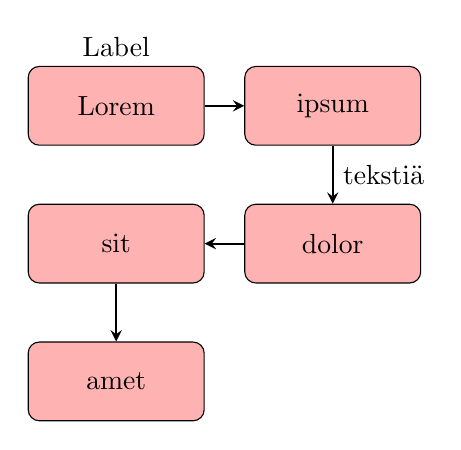
\begin{tikzpicture}[node distance=2.75cm]
\node[label=90:Label] (yksi) [palikka] {Lorem};
\node (kaksi) [palikka, right of=yksi] {ipsum};
\node (kolme) [palikka, below of=kaksi,  yshift=1cm] {dolor};
\node (neljä) [palikka, left of=kolme] {sit};
\node (viisi) [palikka, below of=neljä, yshift=1cm] {amet};
\draw [arrow] (yksi) -- (kaksi);
\draw [arrow] (kaksi) -- node[anchor=west] {tekstiä} (kolme);
\draw [arrow] (kolme) -- (neljä);
\draw [arrow] (neljä) -- (viisi);
\end{tikzpicture}
\caption{Example tikz-picture}
\label{fig:tikz}
\end{figure}

As seen in figure \ref{fig:tikz}, ut porttitor elit sit amet justo dignissim sit amet sagittis massa egestas. Mauris sed dolor eget dui fermentum sodales ut eu nibh. 

\section{Section}

Lorem ipsum dolor sit amet, consectetur adipiscing elit. Aliquam aliquam aliquam purus, in ornare nulla imperdiet molestie. Nam tempus erat eu dui rhoncus et vestibulum mi elementum. Ut porttitor elit sit amet justo dignissim sit amet sagittis massa egestas. Mauris sed dolor eget dui fermentum sodales ut eu nibh. 

\clearpage %force the next chapter to start on a new page. Keep that as the last line of your chapter!
